\batchmode
\documentclass[twoside]{book}

% Packages required by doxygen
\usepackage{fixltx2e}
\usepackage{calc}
\usepackage{doxygen}
\usepackage[export]{adjustbox} % also loads graphicx
\usepackage{graphicx}
\usepackage[utf8]{inputenc}
\usepackage{makeidx}
\usepackage{multicol}
\usepackage{multirow}
\PassOptionsToPackage{warn}{textcomp}
\usepackage{textcomp}
\usepackage[nointegrals]{wasysym}
\usepackage[table]{xcolor}

% Font selection
\usepackage[T1]{fontenc}
\usepackage[scaled=.90]{helvet}
\usepackage{courier}
\usepackage{amssymb}
\usepackage{sectsty}
\renewcommand{\familydefault}{\sfdefault}
\allsectionsfont{%
  \fontseries{bc}\selectfont%
  \color{darkgray}%
}
\renewcommand{\DoxyLabelFont}{%
  \fontseries{bc}\selectfont%
  \color{darkgray}%
}
\newcommand{\+}{\discretionary{\mbox{\scriptsize$\hookleftarrow$}}{}{}}

% Page & text layout
\usepackage{geometry}
\geometry{%
  a4paper,%
  top=2.5cm,%
  bottom=2.5cm,%
  left=2.5cm,%
  right=2.5cm%
}
\tolerance=750
\hfuzz=15pt
\hbadness=750
\setlength{\emergencystretch}{15pt}
\setlength{\parindent}{0cm}
\setlength{\parskip}{3ex plus 2ex minus 2ex}
\makeatletter
\renewcommand{\paragraph}{%
  \@startsection{paragraph}{4}{0ex}{-1.0ex}{1.0ex}{%
    \normalfont\normalsize\bfseries\SS@parafont%
  }%
}
\renewcommand{\subparagraph}{%
  \@startsection{subparagraph}{5}{0ex}{-1.0ex}{1.0ex}{%
    \normalfont\normalsize\bfseries\SS@subparafont%
  }%
}
\makeatother

% Headers & footers
\usepackage{fancyhdr}
\pagestyle{fancyplain}
\fancyhead[LE]{\fancyplain{}{\bfseries\thepage}}
\fancyhead[CE]{\fancyplain{}{}}
\fancyhead[RE]{\fancyplain{}{\bfseries\leftmark}}
\fancyhead[LO]{\fancyplain{}{\bfseries\rightmark}}
\fancyhead[CO]{\fancyplain{}{}}
\fancyhead[RO]{\fancyplain{}{\bfseries\thepage}}
\fancyfoot[LE]{\fancyplain{}{}}
\fancyfoot[CE]{\fancyplain{}{}}
\fancyfoot[RE]{\fancyplain{}{\bfseries\scriptsize Generated by Doxygen }}
\fancyfoot[LO]{\fancyplain{}{\bfseries\scriptsize Generated by Doxygen }}
\fancyfoot[CO]{\fancyplain{}{}}
\fancyfoot[RO]{\fancyplain{}{}}
\renewcommand{\footrulewidth}{0.4pt}
\renewcommand{\chaptermark}[1]{%
  \markboth{#1}{}%
}
\renewcommand{\sectionmark}[1]{%
  \markright{\thesection\ #1}%
}

% Indices & bibliography
\usepackage{natbib}
\usepackage[titles]{tocloft}
\setcounter{tocdepth}{3}
\setcounter{secnumdepth}{5}
\makeindex

% Hyperlinks (required, but should be loaded last)
\usepackage{ifpdf}
\ifpdf
  \usepackage[pdftex,pagebackref=true]{hyperref}
\else
  \usepackage[ps2pdf,pagebackref=true]{hyperref}
\fi
\hypersetup{%
  colorlinks=true,%
  linkcolor=blue,%
  citecolor=blue,%
  unicode%
}

% Custom commands
\newcommand{\clearemptydoublepage}{%
  \newpage{\pagestyle{empty}\cleardoublepage}%
}

\usepackage{caption}
\captionsetup{labelsep=space,justification=centering,font={bf},singlelinecheck=off,skip=4pt,position=top}

%===== C O N T E N T S =====

\begin{document}

% Titlepage & ToC
\hypersetup{pageanchor=false,
             bookmarksnumbered=true
            }
\pagenumbering{alph}
\pagenumbering{arabic}
\hypersetup{pageanchor=true}

%--- Begin generated contents ---
\chapter{Example problem\+: Spin-\/up of a viscous fluid}
\label{index}\hypertarget{index}{}\hypertarget{index_q}{}\section{A few quick questions...}\label{index_q}
Since {\ttfamily oomph-\/lib} is developed as open-\/source software, any evidence that the code is being downloaded and used is very helpful for us as it helps to justify our continued work on this project.

We would therefore be extremely grateful if you could provide the information requested in the form below. Pressing the \char`\"{}submit\char`\"{} button will get you to the actual download page.

{\bfseries Note\+:} 
\begin{DoxyItemize}
\item All information will be treated as confidential. 
\item If you provide your email address and check the appropriate box we will add you to our mailing list to inform you of upgrades and bug fixes to the code. Rest assured that the mailing list is {\bfseries very low volume} -- we have better things to do than to bombard you with email. 
\item If you still feel reluctant to provide any of the information requested, feel free to enter some dummy input. The form will check that {\bfseries some} information has been entered but entering your name as \char`\"{}\+Joe Cool\char`\"{} is perfectly acceptable -- this is to discourage people from not providing the information simply because they are too lazy to type... 
\end{DoxyItemize}



 







 

 \hypertarget{index_pdf}{}\section{P\+D\+F file}\label{index_pdf}
A \href{../latex/refman.pdf}{\tt pdf version} of this document is available. \end{document}

\chapter{Namespace Index}
\section{Namespace List}
Here is a list of all namespaces with brief descriptions\+:\begin{DoxyCompactList}
\item\contentsline{section}{\hyperlink{namespaceGlobal__Physical__Variables}{Global\+\_\+\+Physical\+\_\+\+Variables} \\*Global variables that represent physical properties }{\pageref{namespaceGlobal__Physical__Variables}}{}
\item\contentsline{section}{\hyperlink{namespaceoomph}{oomph} }{\pageref{namespaceoomph}}{}
\item\contentsline{section}{\hyperlink{namespacePhysical__Variables}{Physical\+\_\+\+Variables} \\*Namespace for the solution of 2D linear shell equation }{\pageref{namespacePhysical__Variables}}{}
\end{DoxyCompactList}

\chapter{Hierarchical Index}
\section{Class Hierarchy}
This inheritance list is sorted roughly, but not completely, alphabetically\+:\begin{DoxyCompactList}
\item Problem\begin{DoxyCompactList}
\item \contentsline{section}{Unstructured\+Solid\+Problem$<$ E\+L\+E\+M\+E\+NT $>$}{\pageref{classUnstructuredSolidProblem}}{}
\end{DoxyCompactList}
\end{DoxyCompactList}

\chapter{Class Index}
\section{Class List}
Here are the classes, structs, unions and interfaces with brief descriptions\+:\begin{DoxyCompactList}
\item\contentsline{section}{\hyperlink{classPMLProblem}{P\+M\+L\+Problem$<$ E\+L\+E\+M\+E\+N\+T $>$} }{\pageref{classPMLProblem}}{}
\item\contentsline{section}{\hyperlink{classGlobalParameters_1_1TestPMLMapping}{Global\+Parameters\+::\+Test\+P\+M\+L\+Mapping} }{\pageref{classGlobalParameters_1_1TestPMLMapping}}{}
\end{DoxyCompactList}

\chapter{File Index}
\section{File List}
Here is a list of all files with brief descriptions\+:\begin{DoxyCompactList}
\item\contentsline{section}{\hyperlink{jeffery__orbit_8cc}{jeffery\+\_\+orbit.\+cc} }{\pageref{jeffery__orbit_8cc}}{}
\item\contentsline{section}{\hyperlink{jeffery__orbit_8txt__doxygenified_8h}{jeffery\+\_\+orbit.\+txt\+\_\+doxygenified.\+h} }{\pageref{jeffery__orbit_8txt__doxygenified_8h}}{}
\item\contentsline{section}{\hyperlink{my__taylor__hood__elements_8h}{my\+\_\+taylor\+\_\+hood\+\_\+elements.\+h} }{\pageref{my__taylor__hood__elements_8h}}{}
\end{DoxyCompactList}

\chapter{Namespace Documentation}
\hypertarget{namespaceGlobal__Physical__Variables}{}\section{Global\+\_\+\+Physical\+\_\+\+Variables Namespace Reference}
\label{namespaceGlobal__Physical__Variables}\index{Global\+\_\+\+Physical\+\_\+\+Variables@{Global\+\_\+\+Physical\+\_\+\+Variables}}


Namespace for physical parameters.  


\subsection*{Functions}
\begin{DoxyCompactItemize}
\item 
Vector$<$ double $>$ \hyperlink{namespaceGlobal__Physical__Variables_afae321364975eb56688ad13abc8ed6b7}{Gravity} (2)
\begin{DoxyCompactList}\small\item\em Gravity vector. \end{DoxyCompactList}\item 
void \hyperlink{namespaceGlobal__Physical__Variables_a87da705b8a46bed337cf5dbdd788b87b}{body\+\_\+force} (const double \&time, const Vector$<$ double $>$ \&x, Vector$<$ double $>$ \&result)
\begin{DoxyCompactList}\small\item\em Functional body force. \end{DoxyCompactList}\item 
void \hyperlink{namespaceGlobal__Physical__Variables_a9780d615ae07c4e00a436ab2973b54e6}{zero\+\_\+body\+\_\+force} (const double \&time, const Vector$<$ double $>$ \&x, Vector$<$ double $>$ \&result)
\begin{DoxyCompactList}\small\item\em Zero functional body force. \end{DoxyCompactList}\end{DoxyCompactItemize}
\subsection*{Variables}
\begin{DoxyCompactItemize}
\item 
double \hyperlink{namespaceGlobal__Physical__Variables_ab814e627d2eb5bc50318879d19ab16b9}{Re} =100
\begin{DoxyCompactList}\small\item\em Reynolds number. \end{DoxyCompactList}\item 
double \hyperlink{namespaceGlobal__Physical__Variables_ab1a845a672b4d74b304639a976dc65c6}{Re\+\_\+inv\+Fr} =100
\begin{DoxyCompactList}\small\item\em Reynolds/\+Froude number. \end{DoxyCompactList}\end{DoxyCompactItemize}


\subsection{Detailed Description}
Namespace for physical parameters. 

\subsection{Function Documentation}
\mbox{\Hypertarget{namespaceGlobal__Physical__Variables_a87da705b8a46bed337cf5dbdd788b87b}\label{namespaceGlobal__Physical__Variables_a87da705b8a46bed337cf5dbdd788b87b}} 
\index{Global\+\_\+\+Physical\+\_\+\+Variables@{Global\+\_\+\+Physical\+\_\+\+Variables}!body\+\_\+force@{body\+\_\+force}}
\index{body\+\_\+force@{body\+\_\+force}!Global\+\_\+\+Physical\+\_\+\+Variables@{Global\+\_\+\+Physical\+\_\+\+Variables}}
\subsubsection{\texorpdfstring{body\+\_\+force()}{body\_force()}}
{\footnotesize\ttfamily void Global\+\_\+\+Physical\+\_\+\+Variables\+::body\+\_\+force (\begin{DoxyParamCaption}\item[{const double \&}]{time,  }\item[{const Vector$<$ double $>$ \&}]{x,  }\item[{Vector$<$ double $>$ \&}]{result }\end{DoxyParamCaption})}



Functional body force. 



Definition at line 62 of file circular\+\_\+driven\+\_\+cavity.\+cc.



References Re\+\_\+inv\+Fr.



Referenced by main().

\mbox{\Hypertarget{namespaceGlobal__Physical__Variables_afae321364975eb56688ad13abc8ed6b7}\label{namespaceGlobal__Physical__Variables_afae321364975eb56688ad13abc8ed6b7}} 
\index{Global\+\_\+\+Physical\+\_\+\+Variables@{Global\+\_\+\+Physical\+\_\+\+Variables}!Gravity@{Gravity}}
\index{Gravity@{Gravity}!Global\+\_\+\+Physical\+\_\+\+Variables@{Global\+\_\+\+Physical\+\_\+\+Variables}}
\subsubsection{\texorpdfstring{Gravity()}{Gravity()}}
{\footnotesize\ttfamily Vector$<$double$>$ Global\+\_\+\+Physical\+\_\+\+Variables\+::\+Gravity (\begin{DoxyParamCaption}\item[{2}]{ }\end{DoxyParamCaption})}



Gravity vector. 



Referenced by main(), and Quarter\+Circle\+Driven\+Cavity\+Problem$<$ E\+L\+E\+M\+E\+N\+T $>$\+::\+Quarter\+Circle\+Driven\+Cavity\+Problem().

\mbox{\Hypertarget{namespaceGlobal__Physical__Variables_a9780d615ae07c4e00a436ab2973b54e6}\label{namespaceGlobal__Physical__Variables_a9780d615ae07c4e00a436ab2973b54e6}} 
\index{Global\+\_\+\+Physical\+\_\+\+Variables@{Global\+\_\+\+Physical\+\_\+\+Variables}!zero\+\_\+body\+\_\+force@{zero\+\_\+body\+\_\+force}}
\index{zero\+\_\+body\+\_\+force@{zero\+\_\+body\+\_\+force}!Global\+\_\+\+Physical\+\_\+\+Variables@{Global\+\_\+\+Physical\+\_\+\+Variables}}
\subsubsection{\texorpdfstring{zero\+\_\+body\+\_\+force()}{zero\_body\_force()}}
{\footnotesize\ttfamily void Global\+\_\+\+Physical\+\_\+\+Variables\+::zero\+\_\+body\+\_\+force (\begin{DoxyParamCaption}\item[{const double \&}]{time,  }\item[{const Vector$<$ double $>$ \&}]{x,  }\item[{Vector$<$ double $>$ \&}]{result }\end{DoxyParamCaption})}



Zero functional body force. 



Definition at line 70 of file circular\+\_\+driven\+\_\+cavity.\+cc.



Referenced by main().



\subsection{Variable Documentation}
\mbox{\Hypertarget{namespaceGlobal__Physical__Variables_ab814e627d2eb5bc50318879d19ab16b9}\label{namespaceGlobal__Physical__Variables_ab814e627d2eb5bc50318879d19ab16b9}} 
\index{Global\+\_\+\+Physical\+\_\+\+Variables@{Global\+\_\+\+Physical\+\_\+\+Variables}!Re@{Re}}
\index{Re@{Re}!Global\+\_\+\+Physical\+\_\+\+Variables@{Global\+\_\+\+Physical\+\_\+\+Variables}}
\subsubsection{\texorpdfstring{Re}{Re}}
{\footnotesize\ttfamily double Global\+\_\+\+Physical\+\_\+\+Variables\+::\+Re =100}



Reynolds number. 



Definition at line 53 of file circular\+\_\+driven\+\_\+cavity.\+cc.



Referenced by Quarter\+Circle\+Driven\+Cavity\+Problem$<$ E\+L\+E\+M\+E\+N\+T $>$\+::\+Quarter\+Circle\+Driven\+Cavity\+Problem().

\mbox{\Hypertarget{namespaceGlobal__Physical__Variables_ab1a845a672b4d74b304639a976dc65c6}\label{namespaceGlobal__Physical__Variables_ab1a845a672b4d74b304639a976dc65c6}} 
\index{Global\+\_\+\+Physical\+\_\+\+Variables@{Global\+\_\+\+Physical\+\_\+\+Variables}!Re\+\_\+inv\+Fr@{Re\+\_\+inv\+Fr}}
\index{Re\+\_\+inv\+Fr@{Re\+\_\+inv\+Fr}!Global\+\_\+\+Physical\+\_\+\+Variables@{Global\+\_\+\+Physical\+\_\+\+Variables}}
\subsubsection{\texorpdfstring{Re\+\_\+inv\+Fr}{Re\_invFr}}
{\footnotesize\ttfamily double Global\+\_\+\+Physical\+\_\+\+Variables\+::\+Re\+\_\+inv\+Fr =100}



Reynolds/\+Froude number. 



Definition at line 56 of file circular\+\_\+driven\+\_\+cavity.\+cc.



Referenced by body\+\_\+force(), and Quarter\+Circle\+Driven\+Cavity\+Problem$<$ E\+L\+E\+M\+E\+N\+T $>$\+::\+Quarter\+Circle\+Driven\+Cavity\+Problem().


\chapter{Class Documentation}
\hypertarget{classRotatingCylinderProblem}{}\section{Rotating\+Cylinder\+Problem$<$ E\+L\+E\+M\+E\+NT, T\+I\+M\+E\+S\+T\+E\+P\+P\+ER $>$ Class Template Reference}
\label{classRotatingCylinderProblem}\index{Rotating\+Cylinder\+Problem$<$ E\+L\+E\+M\+E\+N\+T, T\+I\+M\+E\+S\+T\+E\+P\+P\+E\+R $>$@{Rotating\+Cylinder\+Problem$<$ E\+L\+E\+M\+E\+N\+T, T\+I\+M\+E\+S\+T\+E\+P\+P\+E\+R $>$}}


Refineable rotating cylinder problem in a rectangular axisymmetric domain.  


Inheritance diagram for Rotating\+Cylinder\+Problem$<$ E\+L\+E\+M\+E\+NT, T\+I\+M\+E\+S\+T\+E\+P\+P\+ER $>$\+:\begin{figure}[H]
\begin{center}
\leavevmode
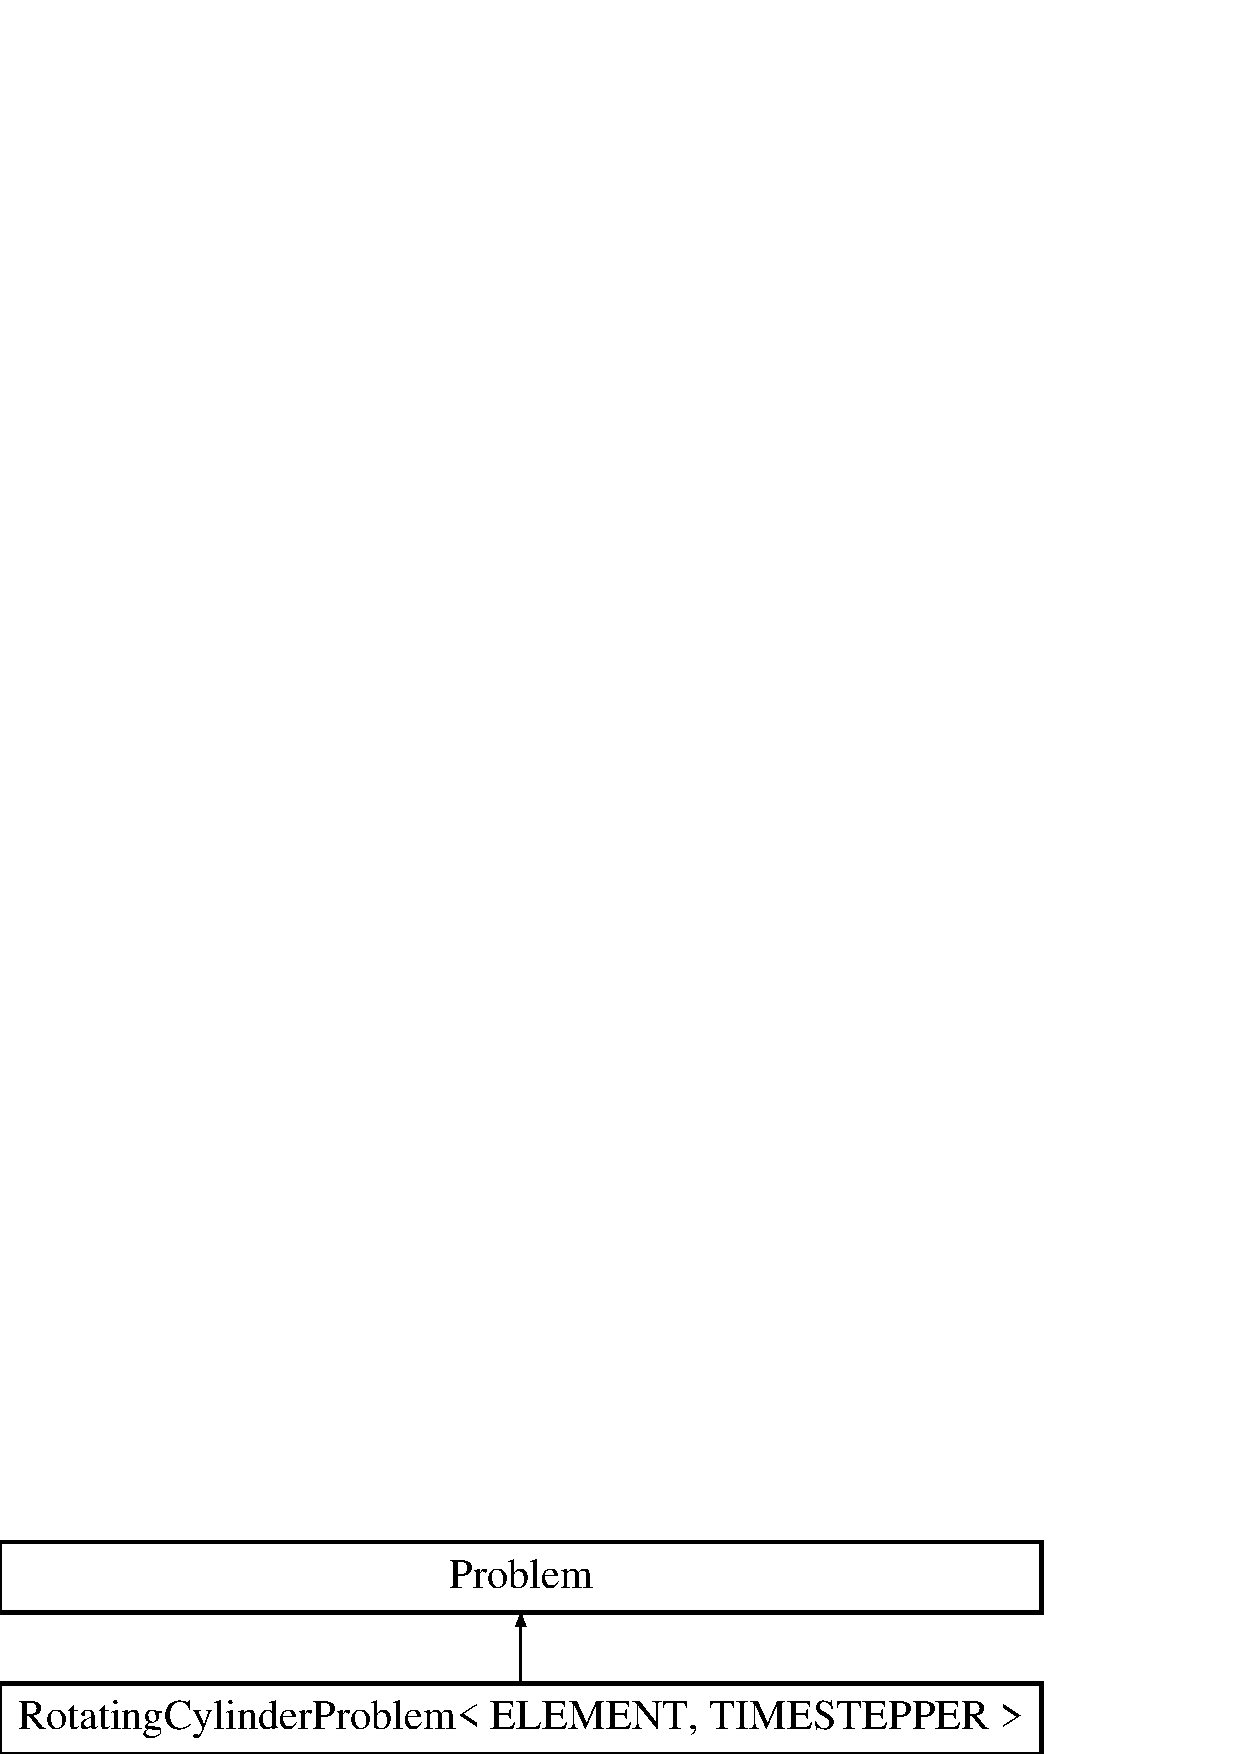
\includegraphics[height=2.000000cm]{classRotatingCylinderProblem}
\end{center}
\end{figure}
\subsection*{Public Member Functions}
\begin{DoxyCompactItemize}
\item 
\hyperlink{classRotatingCylinderProblem_a436b0ff8c4ac33acfe10492c587ad80d}{Rotating\+Cylinder\+Problem} (const unsigned \&n\+\_\+r, const unsigned \&n\+\_\+z, const double \&l\+\_\+r, const double \&l\+\_\+z)
\begin{DoxyCompactList}\small\item\em Constructor for refineable rotating cylinder problem. \end{DoxyCompactList}\item 
\hyperlink{classRotatingCylinderProblem_a586e71f48ee21cfc3bc93d17e91bbc11}{$\sim$\+Rotating\+Cylinder\+Problem} ()
\begin{DoxyCompactList}\small\item\em Destructor (empty) \end{DoxyCompactList}\item 
void \hyperlink{classRotatingCylinderProblem_a5e4316cce2306c4aab4a20b88cdfe6e3}{set\+\_\+initial\+\_\+condition} ()
\begin{DoxyCompactList}\small\item\em Set initial conditions. \end{DoxyCompactList}\item 
void \hyperlink{classRotatingCylinderProblem_a37efdb2d7059535a48b12f69869996ee}{set\+\_\+boundary\+\_\+conditions} ()
\begin{DoxyCompactList}\small\item\em Set boundary conditions. \end{DoxyCompactList}\item 
void \hyperlink{classRotatingCylinderProblem_a22f82fba41d68b9748642f9a29a12592}{doc\+\_\+solution} (Doc\+Info \&doc\+\_\+info)
\begin{DoxyCompactList}\small\item\em Document the solution. \end{DoxyCompactList}\item 
void \hyperlink{classRotatingCylinderProblem_abfb7f77b97e9ac061edbaa97a018cd24}{unsteady\+\_\+run} (const double \&t\+\_\+max, const double \&dt, const string dir\+\_\+name)
\begin{DoxyCompactList}\small\item\em Do unsteady run up to maximum time t\+\_\+max with given timestep dt. \end{DoxyCompactList}\item 
Refineable\+Rectangular\+Quad\+Mesh$<$ E\+L\+E\+M\+E\+NT $>$ $\ast$ \hyperlink{classRotatingCylinderProblem_a49ac12439c31baa10b6a014a8161f78e}{mesh\+\_\+pt} ()
\begin{DoxyCompactList}\small\item\em Access function for the specific mesh. \end{DoxyCompactList}\end{DoxyCompactItemize}
\subsection*{Private Member Functions}
\begin{DoxyCompactItemize}
\item 
void \hyperlink{classRotatingCylinderProblem_af6678f4329624865484d52058d8902a3}{actions\+\_\+before\+\_\+newton\+\_\+solve} ()
\begin{DoxyCompactList}\small\item\em Update the problem specs before solve. Reset velocity boundary conditions just to be on the safe side... \end{DoxyCompactList}\item 
void \hyperlink{classRotatingCylinderProblem_a2cac6acd0607a98fd1b5f2c155335dbd}{actions\+\_\+after\+\_\+newton\+\_\+solve} ()
\begin{DoxyCompactList}\small\item\em No actions required after solve step. \end{DoxyCompactList}\item 
void \hyperlink{classRotatingCylinderProblem_a7d2fc60789ca6e2458be45b94ee40a1c}{actions\+\_\+after\+\_\+adapt} ()
\begin{DoxyCompactList}\small\item\em After adaptation\+: Pin pressure again (the previously pinned value might have disappeared) and pin redudant pressure dofs. \end{DoxyCompactList}\item 
void \hyperlink{classRotatingCylinderProblem_a06a4c2a32a64bb6c0e6cf7a9e3bba157}{fix\+\_\+pressure} (const unsigned \&e, const unsigned \&pdof, const double \&pvalue)
\begin{DoxyCompactList}\small\item\em Fix pressure in element e at pressure dof pdof and set to pvalue. \end{DoxyCompactList}\end{DoxyCompactItemize}


\subsection{Detailed Description}
\subsubsection*{template$<$class E\+L\+E\+M\+E\+NT, class T\+I\+M\+E\+S\+T\+E\+P\+P\+ER$>$\newline
class Rotating\+Cylinder\+Problem$<$ E\+L\+E\+M\+E\+N\+T, T\+I\+M\+E\+S\+T\+E\+P\+P\+E\+R $>$}

Refineable rotating cylinder problem in a rectangular axisymmetric domain. 

Definition at line 75 of file spin\+\_\+up.\+cc.



\subsection{Constructor \& Destructor Documentation}
\mbox{\Hypertarget{classRotatingCylinderProblem_a436b0ff8c4ac33acfe10492c587ad80d}\label{classRotatingCylinderProblem_a436b0ff8c4ac33acfe10492c587ad80d}} 
\index{Rotating\+Cylinder\+Problem@{Rotating\+Cylinder\+Problem}!Rotating\+Cylinder\+Problem@{Rotating\+Cylinder\+Problem}}
\index{Rotating\+Cylinder\+Problem@{Rotating\+Cylinder\+Problem}!Rotating\+Cylinder\+Problem@{Rotating\+Cylinder\+Problem}}
\subsubsection{\texorpdfstring{Rotating\+Cylinder\+Problem()}{RotatingCylinderProblem()}}
{\footnotesize\ttfamily template$<$class E\+L\+E\+M\+E\+NT , class T\+I\+M\+E\+S\+T\+E\+P\+P\+ER $>$ \\
\hyperlink{classRotatingCylinderProblem}{Rotating\+Cylinder\+Problem}$<$ E\+L\+E\+M\+E\+NT, T\+I\+M\+E\+S\+T\+E\+P\+P\+ER $>$\+::\hyperlink{classRotatingCylinderProblem}{Rotating\+Cylinder\+Problem} (\begin{DoxyParamCaption}\item[{const unsigned \&}]{n\+\_\+r,  }\item[{const unsigned \&}]{n\+\_\+z,  }\item[{const double \&}]{l\+\_\+r,  }\item[{const double \&}]{l\+\_\+z }\end{DoxyParamCaption})}



Constructor for refineable rotating cylinder problem. 

Constructor\+: Pass the number of elements and the lengths of the domain in the radial (r) and axial (z) directions 

Definition at line 153 of file spin\+\_\+up.\+cc.



References Global\+\_\+\+Physical\+\_\+\+Variables\+::\+Re, and Global\+\_\+\+Physical\+\_\+\+Variables\+::\+Re\+St.



Referenced by Rotating\+Cylinder\+Problem$<$ E\+L\+E\+M\+E\+N\+T, T\+I\+M\+E\+S\+T\+E\+P\+P\+E\+R $>$\+::fix\+\_\+pressure().

\mbox{\Hypertarget{classRotatingCylinderProblem_a586e71f48ee21cfc3bc93d17e91bbc11}\label{classRotatingCylinderProblem_a586e71f48ee21cfc3bc93d17e91bbc11}} 
\index{Rotating\+Cylinder\+Problem@{Rotating\+Cylinder\+Problem}!````~Rotating\+Cylinder\+Problem@{$\sim$\+Rotating\+Cylinder\+Problem}}
\index{````~Rotating\+Cylinder\+Problem@{$\sim$\+Rotating\+Cylinder\+Problem}!Rotating\+Cylinder\+Problem@{Rotating\+Cylinder\+Problem}}
\subsubsection{\texorpdfstring{$\sim$\+Rotating\+Cylinder\+Problem()}{~RotatingCylinderProblem()}}
{\footnotesize\ttfamily template$<$class E\+L\+E\+M\+E\+NT , class T\+I\+M\+E\+S\+T\+E\+P\+P\+ER $>$ \\
\hyperlink{classRotatingCylinderProblem}{Rotating\+Cylinder\+Problem}$<$ E\+L\+E\+M\+E\+NT, T\+I\+M\+E\+S\+T\+E\+P\+P\+ER $>$\+::$\sim$\hyperlink{classRotatingCylinderProblem}{Rotating\+Cylinder\+Problem} (\begin{DoxyParamCaption}{ }\end{DoxyParamCaption})\hspace{0.3cm}{\ttfamily [inline]}}



Destructor (empty) 



Definition at line 86 of file spin\+\_\+up.\+cc.



\subsection{Member Function Documentation}
\mbox{\Hypertarget{classRotatingCylinderProblem_a7d2fc60789ca6e2458be45b94ee40a1c}\label{classRotatingCylinderProblem_a7d2fc60789ca6e2458be45b94ee40a1c}} 
\index{Rotating\+Cylinder\+Problem@{Rotating\+Cylinder\+Problem}!actions\+\_\+after\+\_\+adapt@{actions\+\_\+after\+\_\+adapt}}
\index{actions\+\_\+after\+\_\+adapt@{actions\+\_\+after\+\_\+adapt}!Rotating\+Cylinder\+Problem@{Rotating\+Cylinder\+Problem}}
\subsubsection{\texorpdfstring{actions\+\_\+after\+\_\+adapt()}{actions\_after\_adapt()}}
{\footnotesize\ttfamily template$<$class E\+L\+E\+M\+E\+NT , class T\+I\+M\+E\+S\+T\+E\+P\+P\+ER $>$ \\
void \hyperlink{classRotatingCylinderProblem}{Rotating\+Cylinder\+Problem}$<$ E\+L\+E\+M\+E\+NT, T\+I\+M\+E\+S\+T\+E\+P\+P\+ER $>$\+::actions\+\_\+after\+\_\+adapt (\begin{DoxyParamCaption}{ }\end{DoxyParamCaption})\hspace{0.3cm}{\ttfamily [inline]}, {\ttfamily [private]}}



After adaptation\+: Pin pressure again (the previously pinned value might have disappeared) and pin redudant pressure dofs. 



Definition at line 119 of file spin\+\_\+up.\+cc.

\mbox{\Hypertarget{classRotatingCylinderProblem_a2cac6acd0607a98fd1b5f2c155335dbd}\label{classRotatingCylinderProblem_a2cac6acd0607a98fd1b5f2c155335dbd}} 
\index{Rotating\+Cylinder\+Problem@{Rotating\+Cylinder\+Problem}!actions\+\_\+after\+\_\+newton\+\_\+solve@{actions\+\_\+after\+\_\+newton\+\_\+solve}}
\index{actions\+\_\+after\+\_\+newton\+\_\+solve@{actions\+\_\+after\+\_\+newton\+\_\+solve}!Rotating\+Cylinder\+Problem@{Rotating\+Cylinder\+Problem}}
\subsubsection{\texorpdfstring{actions\+\_\+after\+\_\+newton\+\_\+solve()}{actions\_after\_newton\_solve()}}
{\footnotesize\ttfamily template$<$class E\+L\+E\+M\+E\+NT , class T\+I\+M\+E\+S\+T\+E\+P\+P\+ER $>$ \\
void \hyperlink{classRotatingCylinderProblem}{Rotating\+Cylinder\+Problem}$<$ E\+L\+E\+M\+E\+NT, T\+I\+M\+E\+S\+T\+E\+P\+P\+ER $>$\+::actions\+\_\+after\+\_\+newton\+\_\+solve (\begin{DoxyParamCaption}{ }\end{DoxyParamCaption})\hspace{0.3cm}{\ttfamily [inline]}, {\ttfamily [private]}}



No actions required after solve step. 



Definition at line 115 of file spin\+\_\+up.\+cc.

\mbox{\Hypertarget{classRotatingCylinderProblem_af6678f4329624865484d52058d8902a3}\label{classRotatingCylinderProblem_af6678f4329624865484d52058d8902a3}} 
\index{Rotating\+Cylinder\+Problem@{Rotating\+Cylinder\+Problem}!actions\+\_\+before\+\_\+newton\+\_\+solve@{actions\+\_\+before\+\_\+newton\+\_\+solve}}
\index{actions\+\_\+before\+\_\+newton\+\_\+solve@{actions\+\_\+before\+\_\+newton\+\_\+solve}!Rotating\+Cylinder\+Problem@{Rotating\+Cylinder\+Problem}}
\subsubsection{\texorpdfstring{actions\+\_\+before\+\_\+newton\+\_\+solve()}{actions\_before\_newton\_solve()}}
{\footnotesize\ttfamily template$<$class E\+L\+E\+M\+E\+NT , class T\+I\+M\+E\+S\+T\+E\+P\+P\+ER $>$ \\
void \hyperlink{classRotatingCylinderProblem}{Rotating\+Cylinder\+Problem}$<$ E\+L\+E\+M\+E\+NT, T\+I\+M\+E\+S\+T\+E\+P\+P\+ER $>$\+::actions\+\_\+before\+\_\+newton\+\_\+solve (\begin{DoxyParamCaption}{ }\end{DoxyParamCaption})\hspace{0.3cm}{\ttfamily [inline]}, {\ttfamily [private]}}



Update the problem specs before solve. Reset velocity boundary conditions just to be on the safe side... 



Definition at line 112 of file spin\+\_\+up.\+cc.

\mbox{\Hypertarget{classRotatingCylinderProblem_a22f82fba41d68b9748642f9a29a12592}\label{classRotatingCylinderProblem_a22f82fba41d68b9748642f9a29a12592}} 
\index{Rotating\+Cylinder\+Problem@{Rotating\+Cylinder\+Problem}!doc\+\_\+solution@{doc\+\_\+solution}}
\index{doc\+\_\+solution@{doc\+\_\+solution}!Rotating\+Cylinder\+Problem@{Rotating\+Cylinder\+Problem}}
\subsubsection{\texorpdfstring{doc\+\_\+solution()}{doc\_solution()}}
{\footnotesize\ttfamily template$<$class E\+L\+E\+M\+E\+NT , class T\+I\+M\+E\+S\+T\+E\+P\+P\+ER $>$ \\
void \hyperlink{classRotatingCylinderProblem}{Rotating\+Cylinder\+Problem}$<$ E\+L\+E\+M\+E\+NT, T\+I\+M\+E\+S\+T\+E\+P\+P\+ER $>$\+::doc\+\_\+solution (\begin{DoxyParamCaption}\item[{Doc\+Info \&}]{doc\+\_\+info }\end{DoxyParamCaption})}



Document the solution. 



Definition at line 324 of file spin\+\_\+up.\+cc.



References Rotating\+Cylinder\+Problem$<$ E\+L\+E\+M\+E\+N\+T, T\+I\+M\+E\+S\+T\+E\+P\+P\+E\+R $>$\+::unsteady\+\_\+run().



Referenced by Rotating\+Cylinder\+Problem$<$ E\+L\+E\+M\+E\+N\+T, T\+I\+M\+E\+S\+T\+E\+P\+P\+E\+R $>$\+::set\+\_\+boundary\+\_\+conditions().

\mbox{\Hypertarget{classRotatingCylinderProblem_a06a4c2a32a64bb6c0e6cf7a9e3bba157}\label{classRotatingCylinderProblem_a06a4c2a32a64bb6c0e6cf7a9e3bba157}} 
\index{Rotating\+Cylinder\+Problem@{Rotating\+Cylinder\+Problem}!fix\+\_\+pressure@{fix\+\_\+pressure}}
\index{fix\+\_\+pressure@{fix\+\_\+pressure}!Rotating\+Cylinder\+Problem@{Rotating\+Cylinder\+Problem}}
\subsubsection{\texorpdfstring{fix\+\_\+pressure()}{fix\_pressure()}}
{\footnotesize\ttfamily template$<$class E\+L\+E\+M\+E\+NT , class T\+I\+M\+E\+S\+T\+E\+P\+P\+ER $>$ \\
void \hyperlink{classRotatingCylinderProblem}{Rotating\+Cylinder\+Problem}$<$ E\+L\+E\+M\+E\+NT, T\+I\+M\+E\+S\+T\+E\+P\+P\+ER $>$\+::fix\+\_\+pressure (\begin{DoxyParamCaption}\item[{const unsigned \&}]{e,  }\item[{const unsigned \&}]{pdof,  }\item[{const double \&}]{pvalue }\end{DoxyParamCaption})\hspace{0.3cm}{\ttfamily [inline]}, {\ttfamily [private]}}



Fix pressure in element e at pressure dof pdof and set to pvalue. 



Definition at line 135 of file spin\+\_\+up.\+cc.



References Rotating\+Cylinder\+Problem$<$ E\+L\+E\+M\+E\+N\+T, T\+I\+M\+E\+S\+T\+E\+P\+P\+E\+R $>$\+::\+Rotating\+Cylinder\+Problem().

\mbox{\Hypertarget{classRotatingCylinderProblem_a49ac12439c31baa10b6a014a8161f78e}\label{classRotatingCylinderProblem_a49ac12439c31baa10b6a014a8161f78e}} 
\index{Rotating\+Cylinder\+Problem@{Rotating\+Cylinder\+Problem}!mesh\+\_\+pt@{mesh\+\_\+pt}}
\index{mesh\+\_\+pt@{mesh\+\_\+pt}!Rotating\+Cylinder\+Problem@{Rotating\+Cylinder\+Problem}}
\subsubsection{\texorpdfstring{mesh\+\_\+pt()}{mesh\_pt()}}
{\footnotesize\ttfamily template$<$class E\+L\+E\+M\+E\+NT , class T\+I\+M\+E\+S\+T\+E\+P\+P\+ER $>$ \\
Refineable\+Rectangular\+Quad\+Mesh$<$E\+L\+E\+M\+E\+NT$>$$\ast$ \hyperlink{classRotatingCylinderProblem}{Rotating\+Cylinder\+Problem}$<$ E\+L\+E\+M\+E\+NT, T\+I\+M\+E\+S\+T\+E\+P\+P\+ER $>$\+::mesh\+\_\+pt (\begin{DoxyParamCaption}{ }\end{DoxyParamCaption})\hspace{0.3cm}{\ttfamily [inline]}}



Access function for the specific mesh. 



Definition at line 102 of file spin\+\_\+up.\+cc.

\mbox{\Hypertarget{classRotatingCylinderProblem_a37efdb2d7059535a48b12f69869996ee}\label{classRotatingCylinderProblem_a37efdb2d7059535a48b12f69869996ee}} 
\index{Rotating\+Cylinder\+Problem@{Rotating\+Cylinder\+Problem}!set\+\_\+boundary\+\_\+conditions@{set\+\_\+boundary\+\_\+conditions}}
\index{set\+\_\+boundary\+\_\+conditions@{set\+\_\+boundary\+\_\+conditions}!Rotating\+Cylinder\+Problem@{Rotating\+Cylinder\+Problem}}
\subsubsection{\texorpdfstring{set\+\_\+boundary\+\_\+conditions()}{set\_boundary\_conditions()}}
{\footnotesize\ttfamily template$<$class E\+L\+E\+M\+E\+NT , class T\+I\+M\+E\+S\+T\+E\+P\+P\+ER $>$ \\
void \hyperlink{classRotatingCylinderProblem}{Rotating\+Cylinder\+Problem}$<$ E\+L\+E\+M\+E\+NT, T\+I\+M\+E\+S\+T\+E\+P\+P\+ER $>$\+::set\+\_\+boundary\+\_\+conditions (\begin{DoxyParamCaption}{ }\end{DoxyParamCaption})}



Set boundary conditions. 

Set boundary conditions\+: Set both velocity components to zero on the bottom (solid) wall and the horizontal component only to zero on the side (periodic) boundaries. 

Definition at line 278 of file spin\+\_\+up.\+cc.



References Rotating\+Cylinder\+Problem$<$ E\+L\+E\+M\+E\+N\+T, T\+I\+M\+E\+S\+T\+E\+P\+P\+E\+R $>$\+::doc\+\_\+solution().

\mbox{\Hypertarget{classRotatingCylinderProblem_a5e4316cce2306c4aab4a20b88cdfe6e3}\label{classRotatingCylinderProblem_a5e4316cce2306c4aab4a20b88cdfe6e3}} 
\index{Rotating\+Cylinder\+Problem@{Rotating\+Cylinder\+Problem}!set\+\_\+initial\+\_\+condition@{set\+\_\+initial\+\_\+condition}}
\index{set\+\_\+initial\+\_\+condition@{set\+\_\+initial\+\_\+condition}!Rotating\+Cylinder\+Problem@{Rotating\+Cylinder\+Problem}}
\subsubsection{\texorpdfstring{set\+\_\+initial\+\_\+condition()}{set\_initial\_condition()}}
{\footnotesize\ttfamily template$<$class E\+L\+E\+M\+E\+NT , class T\+I\+M\+E\+S\+T\+E\+P\+P\+ER $>$ \\
void \hyperlink{classRotatingCylinderProblem}{Rotating\+Cylinder\+Problem}$<$ E\+L\+E\+M\+E\+NT, T\+I\+M\+E\+S\+T\+E\+P\+P\+ER $>$\+::set\+\_\+initial\+\_\+condition (\begin{DoxyParamCaption}{ }\end{DoxyParamCaption})}



Set initial conditions. 

Set initial conditions\+: Set all nodal velocities to zero and initialise the previous velocities to correspond to an impulsive start. 

Definition at line 248 of file spin\+\_\+up.\+cc.

\mbox{\Hypertarget{classRotatingCylinderProblem_abfb7f77b97e9ac061edbaa97a018cd24}\label{classRotatingCylinderProblem_abfb7f77b97e9ac061edbaa97a018cd24}} 
\index{Rotating\+Cylinder\+Problem@{Rotating\+Cylinder\+Problem}!unsteady\+\_\+run@{unsteady\+\_\+run}}
\index{unsteady\+\_\+run@{unsteady\+\_\+run}!Rotating\+Cylinder\+Problem@{Rotating\+Cylinder\+Problem}}
\subsubsection{\texorpdfstring{unsteady\+\_\+run()}{unsteady\_run()}}
{\footnotesize\ttfamily template$<$class E\+L\+E\+M\+E\+NT , class T\+I\+M\+E\+S\+T\+E\+P\+P\+ER $>$ \\
void \hyperlink{classRotatingCylinderProblem}{Rotating\+Cylinder\+Problem}$<$ E\+L\+E\+M\+E\+NT, T\+I\+M\+E\+S\+T\+E\+P\+P\+ER $>$\+::unsteady\+\_\+run (\begin{DoxyParamCaption}\item[{const double \&}]{t\+\_\+max,  }\item[{const double \&}]{dt,  }\item[{const string}]{dir\+\_\+name }\end{DoxyParamCaption})}



Do unsteady run up to maximum time t\+\_\+max with given timestep dt. 

Perform run up to specified time t\+\_\+max with given timestep dt. 

Definition at line 356 of file spin\+\_\+up.\+cc.



Referenced by Rotating\+Cylinder\+Problem$<$ E\+L\+E\+M\+E\+N\+T, T\+I\+M\+E\+S\+T\+E\+P\+P\+E\+R $>$\+::doc\+\_\+solution().



The documentation for this class was generated from the following file\+:\begin{DoxyCompactItemize}
\item 
\hyperlink{spin__up_8cc}{spin\+\_\+up.\+cc}\end{DoxyCompactItemize}

\chapter{File Documentation}
\hypertarget{spin__up_8cc}{}\section{spin\+\_\+up.\+cc File Reference}
\label{spin__up_8cc}\index{spin\+\_\+up.\+cc@{spin\+\_\+up.\+cc}}
\subsection*{Classes}
\begin{DoxyCompactItemize}
\item 
class \hyperlink{classRotatingCylinderProblem}{Rotating\+Cylinder\+Problem$<$ E\+L\+E\+M\+E\+N\+T, T\+I\+M\+E\+S\+T\+E\+P\+P\+E\+R $>$}
\begin{DoxyCompactList}\small\item\em Refineable rotating cylinder problem in a rectangular axisymmetric domain. \end{DoxyCompactList}\end{DoxyCompactItemize}
\subsection*{Namespaces}
\begin{DoxyCompactItemize}
\item 
 \hyperlink{namespaceGlobal__Physical__Variables}{Global\+\_\+\+Physical\+\_\+\+Variables}
\begin{DoxyCompactList}\small\item\em Namespace for physical parameters. \end{DoxyCompactList}\end{DoxyCompactItemize}
\subsection*{Functions}
\begin{DoxyCompactItemize}
\item 
int \hyperlink{spin__up_8cc_a0ddf1224851353fc92bfbff6f499fa97}{main} (int argc, char $\ast$argv\mbox{[}$\,$\mbox{]})
\begin{DoxyCompactList}\small\item\em Driver code for axisymmetric spin-\/up problem. \end{DoxyCompactList}\end{DoxyCompactItemize}
\subsection*{Variables}
\begin{DoxyCompactItemize}
\item 
double \hyperlink{namespaceGlobal__Physical__Variables_ab814e627d2eb5bc50318879d19ab16b9}{Global\+\_\+\+Physical\+\_\+\+Variables\+::\+Re} = 5.\+0
\begin{DoxyCompactList}\small\item\em Reynolds number. \end{DoxyCompactList}\item 
double \hyperlink{namespaceGlobal__Physical__Variables_a085ee4bf968ffdd01a41b8c41864f907}{Global\+\_\+\+Physical\+\_\+\+Variables\+::\+Re\+St} = 5.\+0
\begin{DoxyCompactList}\small\item\em Womersley number. \end{DoxyCompactList}\end{DoxyCompactItemize}


\subsection{Function Documentation}
\mbox{\Hypertarget{spin__up_8cc_a0ddf1224851353fc92bfbff6f499fa97}\label{spin__up_8cc_a0ddf1224851353fc92bfbff6f499fa97}} 
\index{spin\+\_\+up.\+cc@{spin\+\_\+up.\+cc}!main@{main}}
\index{main@{main}!spin\+\_\+up.\+cc@{spin\+\_\+up.\+cc}}
\subsubsection{\texorpdfstring{main()}{main()}}
{\footnotesize\ttfamily int main (\begin{DoxyParamCaption}\item[{int}]{argc,  }\item[{char $\ast$}]{argv\mbox{[}$\,$\mbox{]} }\end{DoxyParamCaption})}



Driver code for axisymmetric spin-\/up problem. 

Maximum time

Duration of timestep 

Definition at line 431 of file spin\+\_\+up.\+cc.


\hypertarget{spin__up_8txt__doxygenified_8h}{}\section{spin\+\_\+up.\+txt\+\_\+doxygenified.\+h File Reference}
\label{spin__up_8txt__doxygenified_8h}\index{spin\+\_\+up.\+txt\+\_\+doxygenified.\+h@{spin\+\_\+up.\+txt\+\_\+doxygenified.\+h}}

%--- End generated contents ---

% Index
\backmatter
\newpage
\phantomsection
\clearemptydoublepage
\addcontentsline{toc}{chapter}{Index}
\printindex

